%%%%%%%%%%%%%%%%%%%%%%%%%%%%%%%%%%%%%%%%%%%%%%%%%%%%%%%%%%%%%%%%%%%%%
%% This is a (brief) model paper using the achemso class
%% The document class accepts keyval options, which should include
%% the target journal and optionally the manuscript type.
%%%%%%%%%%%%%%%%%%%%%%%%%%%%%%%%%%%%%%%%%%%%%%%%%%%%%%%%%%%%%%%%%%%%%
\documentclass[journal=jctcce,manuscript=article]{achemso}
\setkeys{acs}{articletitle=false}

%%%%%%%%%%%%%%%%%%%%%%%%%%%%%%%%%%%%%%%%%%%%%%%%%%%%%%%%%%%%%%%%%%%%%
%% Place any additional packages needed here.  Only include packages
%% which are essential, to avoid problems later. Do NOT use any
%% packages which require e-TeX (for example etoolbox): the e-TeX
%% extensions are not currently available on the ACS conversion
%% servers.
%%%%%%%%%%%%%%%%%%%%%%%%%%%%%%%%%%%%%%%%%%%%%%%%%%%%%%%%%%%%%%%%%%%%%
\usepackage[version=3]{mhchem} % Formula subscripts using \ce{}
\usepackage{chemnum}
\usepackage{multirow}
\usepackage{textgreek}
\usepackage{textcomp}
\usepackage{setspace}
\usepackage{afterpage}

\usepackage{makecell}

\usepackage{dblfloatfix}


\usepackage{natbib}
\usepackage[acroymn]{glossaries}
\usepackage{tabularx} % for 'tabularx' environment
\usepackage{array}

\usepackage{acro}

\acsetup{hyperref=true}

\usepackage{enumitem}

\usepackage{multicol}
\usepackage{graphicx}
\usepackage{subcaption}

% glossary
\usepackage{hyperref}


\hypersetup{
    colorlinks,
    citecolor=black,
    filecolor=black,
    linkcolor=black,
    urlcolor=black
}



%%%%%%%%%%%%%%%%%%%%%%%%%%%%%%%%%%%%%%%%%%%%%%%%%%%%%%%%%%%%%%%%%%%%%
%% If issues arise when submitting your manuscript, you may want to
%% un-comment the next line.  This provides information on the
%% version of every file you have used.
%%%%%%%%%%%%%%%%%%%%%%%%%%%%%%%%%%%%%%%%%%%%%%%%%%%%%%%%%%%%%%%%%%%%%
%%\listfiles

%%%%%%%%%%%%%%%%%%%%%%%%%%%%%%%%%%%%%%%%%%%%%%%%%%%%%%%%%%%%%%%%%%%%%
%% Place any additional macros here.  Please use \newcommand* where
%% possible, and avoid layout-changing macros (which are not used
%% when typesetting).
%%%%%%%%%%%%%%%%%%%%%%%%%%%%%%%%%%%%%%%%%%%%%%%%%%%%%%%%%%%%%%%%%%%%%
\newcommand*\mycommand[1]{\texttt{\emph{#1}}}

%%%%%%%%%%%%%%%%%%%%%%%%%%%%%%%%%%%%%%%%%%%%%%%%%%%%%%%%%%%%%%%%%%%%%
%% Meta-data block
%% ---------------
%% Each author should be given as a separate \author command.
%%
%% Corresponding authors should have an e-mail given after the author
%% name as an \email command. Phone and fax numbers can be given
%% using \phone and \fax, respectively; this information is optional.
%%
%% The affiliation of authors is given after the authors; each
%% \affiliation command applies to all preceding authors not already
%% assigned an affiliation.
%%
%% The affiliation takes an option argument for the short name.  This
%% will typically be something like "University of Somewhere".
%%
%% The \altaffiliation macro should be used for new address, etc.
%% On the other hand, \alsoaffiliation is used on a per author basis
%% when authors are associated with multiple institutions.
%%%%%%%%%%%%%%%%%%%%%%%%%%%%%%%%%%%%%%%%%%%%%%%%%%%%%%%%%%%%%%%%%%%%%
\author{Eric D. Boittier}
\email{eric.boittier@uqconnect.edu.au}
\affiliation[UQ]{The University of Queendland, St Lucia, Queensland, Australia}

\author{\linebreak Supervisors: A/Professor Vito Ferro}
\affiliation[UQ]{The University of Queendland, St Lucia, Queensland, Australia}

\author{Dr Neha Gandhi}
\affiliation[QUT]{Queensland University of Technology, Gardens Point, Queensland, Australia}


%%%%%%%%%%%%%%%%%%%%%%%%%%%%%%%%%%%%%%%%%%%%%%%%%%%%%%%%%%%%%%%%%%%%%
%% The document title should be given as usual. Some journals require
%% a running title from the author: this should be supplied as an
%% optional argument to \title.
%%%%%%%%%%%%%%%%%%%%%%%%%%%%%%%%%%%%%%%%%%%%%%%%%%%%%%%%%%%%%%%%%%%%%
\title[Honours]
  {Parameterisation of ``VinaCarb" for improved docking of heparin/heparan sulfate  \linebreak \large Research Proposal}

%%%%%%%%%%%%%%%%%%%%%%%%%%%%%%%%%%%%%%%%%%%%%%%%%%%%%%%%%%%%%%%%%%%%%
%% Some journals require a list of abbreviations or keywords to be
%% supplied. These should be set up here, and will be printed after
%% the title and author information, if needed.
%%%%%%%%%%%%%%%%%%%%%%%%%%%%%%%%%%%%%%%%%%%%%%%%%%%%%%%%%%%%%%%%%%%%%
\abbreviations{IR,NMR,UV}
\keywords{American Chemical Society}

\DeclareAcronym{Ido}{
    short = IdoA ,
    long = {\small L}-iduronic acid
}

\DeclareAcronym{Glc}{
    short = Glc ,
    long = {\small D}-glucose
}

\DeclareAcronym{Gal}{
    short = Gal ,
    long = {\small D}-galactose
}

\DeclareAcronym{DFT}{
    short = DFT ,
    long = density functional theory
}

\DeclareAcronym{GlcN}{
    short = GlcN ,
    long = {\small D}-glucosamine
}

% \DeclareAcronym{GalA}{
%     short = GalA ,
%     long = {\small D}-galacturonic acid
% }

\DeclareAcronym{GlcA}{
    short = GlcA ,
    long = {\small D}-glucuronic acid
}

\DeclareAcronym{GalN}{
    short = GalN ,
    long = {\small D}-galactosamine
}

\DeclareAcronym{GlcNAc}{
    short = GlcNAc ,
    long = N-acetyl-{\small D}-glucosamine
}

\DeclareAcronym{PG}{
    short = PG ,
    long = proteoglycan
}

\DeclareAcronym{ECM}{
    short = ECM ,
    long = extracellular matrix
}

\DeclareAcronym{GAG}{
    short = GAG ,
    long = glycosaminoglycan
}

\DeclareAcronym{Hep}{
    short = Hep ,
    long = heparin
}
\DeclareAcronym{HS}{
    short = HS ,
    long = heparan sulfate
}
\DeclareAcronym{HA}{
    short = HA ,
    long = hyaluronic acid
}
\DeclareAcronym{CS}{
    short = CS,
    long = chondroitin sulfate
}
\DeclareAcronym{KS}{
    short = KS,
    long = keteran sulfate
}
\DeclareAcronym{DS}{
    short = DS,
    long = dermatin sulfate
}


\DeclareAcronym{DoS}{
    short = DoS,
    long = degree of sulfation
}

\DeclareAcronym{SNFG}{
    short = SNFG, 
    long = structural nomenclature for glycans
}


\DeclareAcronym{APP}{
    short = APP,
    long = amyloid precursor protein
}
\DeclareAcronym{Al}{
    short = APP,
    long = amyloid precursor protein
}
\DeclareAcronym{QM}{
    short = QM,
    long = quantum mechanics
}
\DeclareAcronym{MD}{
    short = MD,
    long = molecular dynamics
}

\DeclareAcronym{FGF1}{
    short = FGF1,
    long = fibroblast growth factor 1
}
\DeclareAcronym{FGF2}{
    short = FGF2,
    long = fibroblast growth factor 2
}
\DeclareAcronym{FGF}{
    short = FGF,
    long = fibroblast growth factor 
}
\DeclareAcronym{AT3}{
    short = ATIII,
    long = \textalpha-antithrombin III
}

\DeclareAcronym{RMSD}{
    short = RMSD,
    long = root mean square deviation
}
\DeclareAcronym{PRMSD}{
    short = PRMSD,
    long = pose root mean square deviation
}

\DeclareAcronym{RBD}{
    short = RBD,
    long = rigid body docking
}

\DeclareAcronym{SAR}{
    short = SAR,
    long = structure activity relationship
}

\newcommand{\squeezeup}{\vspace{-2.5mm}}


\begin{document}


%%%%%%%%%%%%%%%%%%%%%%%%%%%%%%%%%%%%%%%%%%%%%%%%%%%%%%%%%%%%%%%%%%%%%
%% The manuscript does not need to include \maketitle, which is
%% executed automatically.  The document should begin with an
%% abstract, if appropriate.  If one is given and should not be, the
%% contents will be gobbled.
%%%%%%%%%%%%%%%%%%%%%%%%%%%%%%%%%%%%%%%%%%%%%%%%%%%%%%%%%%%%%%%%%%%%%
{\setstretch{1.5} 
\renewcommand{\contentsname}{Table of Contents}

\renewcommand{\thesubfigure}{\Alph{subfigure}}

\newpage
\tableofcontents
\newpage
\listoffigures
\newpage
\listoftables
\newpage
\begin{multicols}{2}
{\setstretch{1}
\printacronyms[name={Abbreviations}, list-style={table}]
}
\end{multicols}

%%%%%%%%%%%%%%%%%%%%%%%%%%%%%%%%%%%%%%%%%%%%%%%%%%%%%%%%%%%%%%%%%%%%%
%% Start the main part of the manuscript here.
%%%%%%%%%%%%%%%%%%%%%%%%%%%%%%%%%%%%%%%%%%%%%%%%%%%%%%%%%%%%%%%%%%%%%
\pagebreak

\section{Background}
\subsection{Heparin and heparan sulfate}

\subsubsection{Structure}

\setlength{\textfloatsep}{0.5cm}
\begin{figure}[!b]
    \begin{subfigure}[b]{0.7\textwidth}
        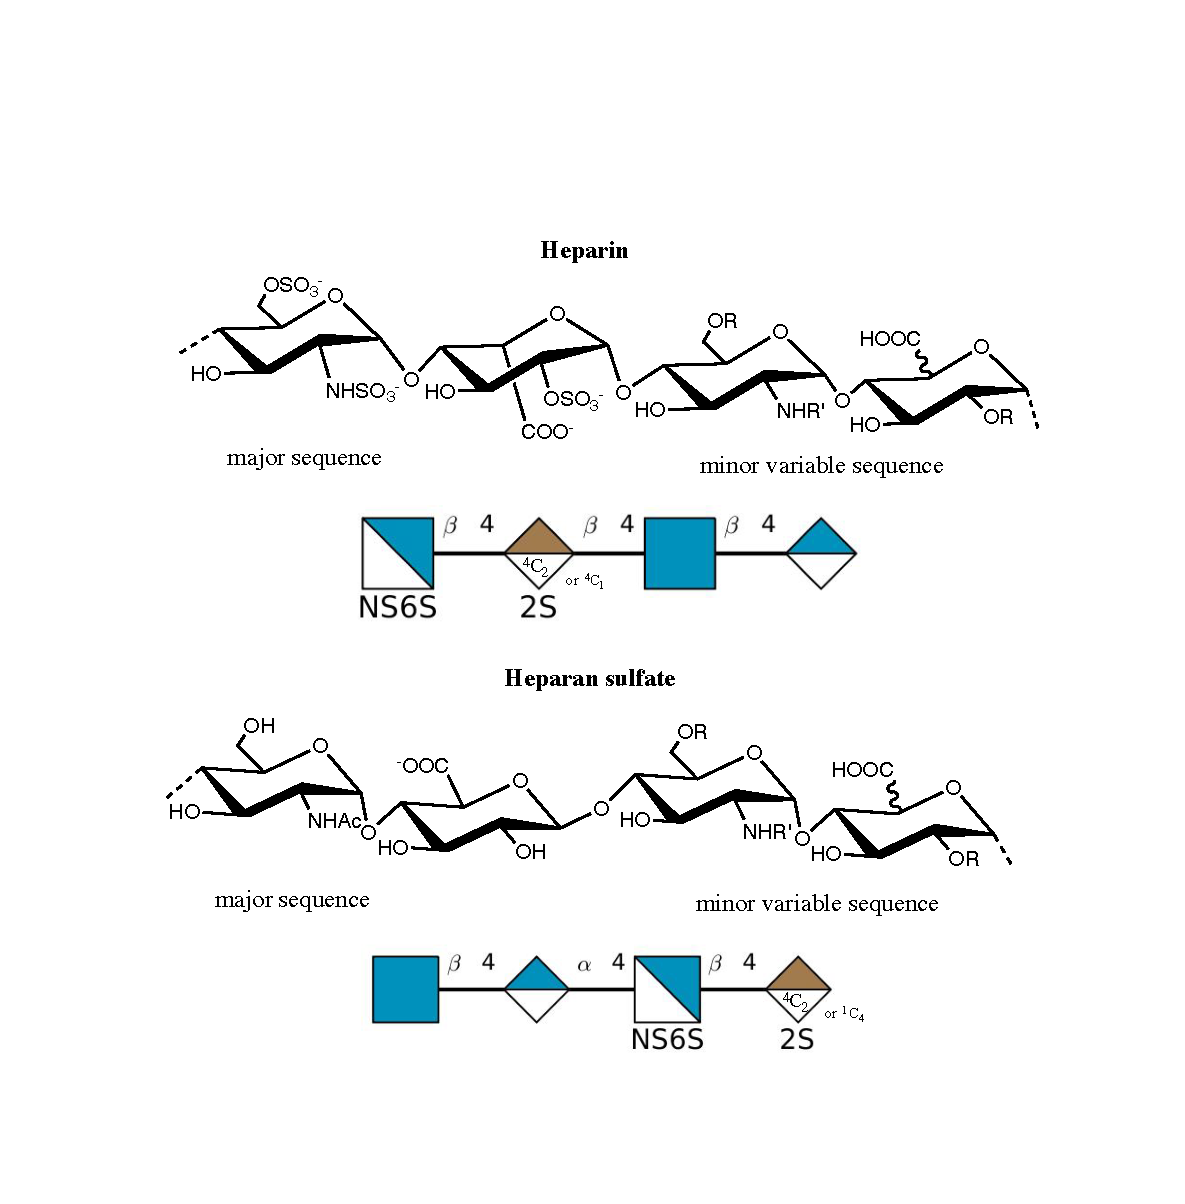
\includegraphics[width=10cm]{heparin_heparan.pdf}
        \caption{}
        \label{fig:HSHep}
    \end{subfigure}
    \begin{subfigure}[b]{0.28\textwidth}
        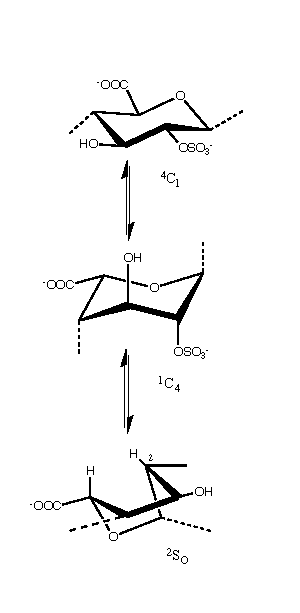
\includegraphics[width=4cm]{ido_confs.pdf}
        \caption{}
        \label{fig:IdoConfs}
    \end{subfigure}
    \caption{The structural and conformations diversity of heparin/heparin sulfate polymers. (A)  (B) Ring conformation equilibrium of iduronic acid.}
\end{figure}

On the surface of all eukariotic cells, highly-sulfated complex polysaccharides known as \acp{GAG} act as emissaries for the reception and modulation of a wide range of proteins, affecting normal physiological processes, such as blood coagulation and neuronal development, as well as serious pathophysiological disorders, such as cancer and Alzhiemer's disease. 
\Ac{Hep} and \ac{HS} are members of the \ac{GAG} family and possess some of the highest negative charge density in all of nature. 
In the clinic, \ac{Hep} is a widely used anticoagulant drug to treat patients with thrombic disorders.\cite{Liu2014ChemoenzymaticHeparin.}
Like all \acp{GAG}, these oligosaccharides are comprised of repeating uronic acid residues (\ac{Ido} or its C5 epimer, \ac{GlcA}, which are \textalpha/\textbeta 1\textrightarrow4-linked, respectively) paired with \textalpha 1\textrightarrow4-linked \ac{GlcN} residues (Figure \ref{fig:HSHep}). 
Each \ac{GAG} can exhibit various sulfation patterns and \ac{DoS} (the number of sulfo groups per disaccharide), which is a product of \textgreater26 proteins involved in \ac{GAG} biosynthesis in the golgi apparatus.\cite{SoaresdaCosta2017SulfationDisorders, Varki2009BiologicalGlycans} 
While \ac{Hep} and \ac{HS} are comprised of similar disaccharide building blocks, their \ac{DoS}, saccharide make up and native location in the cell varies.
\ac{Hep} has higher sulfation levels than HS (\ac{DoS} 2.6 vs 0.6, respectively). 
Upregulation of \ac{Ido} also varies; around 9 in 10 of the disaccharide units in \ac{Hep} contain \ac{Ido}, while only 2 in 10 \ac{HS} disaccharide units contain \ac{Ido}. While \ac{HS} occurs in many cell types, heparin is isolated exclusively from mast cells.\cite{Liu2014ChemoenzymaticHeparin., Gandhi2008TheProteins}

%%%%
% 
%%%%

The structural encoding ability of \acp{GAG} rivals that of DNA, RNA and proteins.\cite{Gama2006SulfationActivity} The amino sugar can be sulphated at C4, C6, the unsubstituted nitrogen or C3 (rare), and the uronic acid residue can be substituted at a variety of positions -- leading to \textgreater1,000,000 possible substitution patterns for a \ac{GAG} octasaccharide.\cite{Gandhi2008TheProteins, SoaresdaCosta2017SulfationDisorders,Gama2006SulfationActivity} GAG sulfation patterns have been likened to the “sulfation code” and multiple \ac{SAR} studies suggest high specificity in relation to function.\cite{Habuchi2004SulfationCode, Gama2006SulfationActivity} Due to this variation, isolating defined sulfation sequences from biological sources is understandably difficult and is often \cite{Gama2006SulfationActivity}. 

Flexible ring conformations of the heparin components add further structural complexity to the oligosaccharide and are reasoned to have bioloigical relevance during \ac{GAG}--protein interactions.\cite{Sattelle2013DoesHeparanome} 
Although \ac{GlcA} and \ac{GlcN} remain in the standard $^{4}C_{1}$ conformation, the exceptional plasticity of \ac{Ido} ring conformations is unique amongst sugars, and is dependent on its position in the chain, ionic conditions and sulfation pattern.\cite{Capila2002Heparin-proteinInteractions., vanBoeckel1987ConformationalAcid}
At the reducing end, \ac{Ido} has been characterized as existing in an equilibrium between $^{4}C_{1}$, $^{1}C_{4}$ and $^{2}S_{O}$, using $^{1}$H NMR spectroscopy (Figure \ref{fig:IdoConfs}).\cite{Ferro1986EvidenceStudies, vanBoeckel1987ConformationalAcid} 
When \ac{Ido} is inside the chain, the equilibrium favors the $^{1}C_{4}$ and $^{2}S_{O}$ conformations exclusively, due to interactions with the 1\textrightarrow4-linked neighbouring sugar.\cite{vanBoeckel1987ConformationalAcid} 
When \ac{Ido} is sulfated at the C2 position, the $^{2}S_{O}$ conformer may become more prominent to minimize unfavorable 1,3 diaxial interactions in the $^{1}C_{4}$ structure.\cite{Hsieh2016UncoveringSulphateb} However, the barrier for interconversion between the two conformers is low and has little effect on the overall conformation of the oligosaccharide, allowing \ac{Ido} to adopt poses suited for specific interactions between basic residues. \cite{Capila2002Heparin-proteinInteractions.} In the case of the \ac{Hep} and \ac{FGF2} complex, two \ac{Ido} residues are poised in $^{1}C_{4}$ and $^{2}S_{O}$ conformations respectively.\cite{Faham1996HeparinFactor} Ring flipping, which is believed to occur on the \textmu s timescale based on \ac{MD} simulations, has been a proposed as mechanism for selective binding/unbinding. \cite{Sattelle2012DependenceIdopyranosides} Standard NMR techniques struggle dramatically to discriminate between the exchange of even the most simple conformers on the \textmu s timescale - at best only 10\% of conformers are perceptible.\cite{Sattelle2011IsChair} Therefore \ac{MD} simulations are crucial to gain insite into these types of structural equilibria.\cite{Woods2018PredictingComplexes} 
For instance, \ac{GlcNAc} was previously assumed to adopt a stable, $^{4}C_{1}$ chair conformation.\cite{Sattelle2011IsChair} 
However, when crystal structures of ligands conatining GlcNAc residues were obtained, conformer deviations to $^{2}S_{O}$ were observed which suggest that the local chemical environment plays an important role in the 3D structure of the sugar. 
\ac{MD} simulations of GlcNAc in solution, over a 20 \textmu s timescale, reached a conformational equilibrium between 3 - 5 \textmu s. 
Although  $^{1}C_{4}$ was the predominant conformer (approx. 99.6\%), the $^{2}S_{O}$ and other minor conformers were also observed.





% PHI and PSI

% Although the overall helical structure is maintained in the
% FGF-bound HSGAG compared with unbound HSGAG, we observe
% distinct changes in the backbone torsion angles of the oligosaccharide
% chain induced upon protein binding. These changes result in local
% deviations in the helical axis that provide optimal ionic and van der
% Waals contact with the protein. A specific conformation and topological
% arrangement of the HSGAG-binding loops of FGF, on the other
% hand, impose structural constraints that induce the local deviations in
% the HSGAG structure, thereby enabling maximum contact between
% HSGAG and the protein.



{\renewcommand{\arraystretch}{1.5}
\setlength{\tabcolsep}{0.3cm}

\begin{table}[bl!]
    \hspace{}
    \begin{tabular}{p{2cm}p{5.5cm}p{7.5cm}}
        \hline
        Technique & Characterization & Disadvantages  \\
        \hline 
        \makecell[tl]{X-ray \\ crystall--\\ography} & 3D structure of ligand--protein complex in a single low energy conformation & \makecell[tl]{\textbullet $ $ Often errors in residue structures/names\\ \textbullet $ $  Only identifies one conformation\\ \textbullet $ $  Protons are not characterized } \\
        
        NMR & Time averaged angles, dihedrals and distance between protons, structural connectivity & 
        \makecell[tl]{\textbullet $ $ Time averaged structure cannot inform \\ \hspace{3mm} structural ensembles\\ \textbullet $ $  Innappropriate for long (\textgreater\textmu s) timescales \\ \textbullet $ $  Small error in coupling constants result \\ \hspace{3mm} in large structural uncertainty }\\ 
    
        \makecell[tl]{Molecular \\ dynamics} & Simulations of the structure of ligand--protein complexes over time & \makecell[tl]{\textbullet $ $ Relies on accurate forcefields and models \\ \textbullet $ $  Computationally expensive for long \\ \hspace{3mm} (\textgreater\textmu s) timescales}  \\
        \hline
        
    \end{tabular}
    \caption{Experimental and \textit{in silico} methods for characterisation of the 3D structure of glycosaminoglycans.}
    \label{tab:GAGprotein}
\end{table}
}




\newpage

\subsubsection{Protein interactions}
{\renewcommand{\arraystretch}{1.5}
\begin{table}[b!]
    \begin{tabular}{p{5cm}p{6cm}p{3cm}}
        \hline
        Heparin--binding protein & Physiological/pathological role & GAG family  \\
        \hline
        AT III & Blood coagulation cascade & Hep 
    \end{tabular}
    \caption{Physiological/pathological effects of Hep/HS--protein interactions.}
    \label{tab:GAGprotein}
\end{table}
}

At physiological pH, all carboxylic acid and sulphate groups are deprotonated. 


\acp{GAG} bind to distinct attachment receptors on proteins such as chemokines, cytokines, growth factors, morphogens, enzymes and adhesion molecules\cite{Murphy2007StructuralHeparin, Iozzo2001HeparanArena, Kreuger2006InteractionsSpecificity, Kowitsch2018MedicalReview}. 

Carbohydrates form hydrogen bonds with side chain residues of polar planar amino acid residues (ASN, ASP, GLY, GLN, ARG and HIS)\cite{Malik2007SequenceNetwork}.
These hydrogen bonds can be cooperative hydrogen bonds, bidentate hydrogen bonds or hydrogen bond networks and facilitate low energy conformations of the polysaccharide.\cite{Quiocho1989Protein-carbohydrateFeatures} 

\ac{HS} and other \acp{GAG} can interact with AB peptides and enhance the shift of AB42 peptides to the \textbeta-sheet confirmation.

\ac{HS} and \ac{Hep} are key to the regulation of Alzheimer's  \textbeta-secretase (BACE1), as they bind to BACE-1 and inhibit cleavage of \ac{APP} and aggregate into amyloid plaques involved with the overall progression of the disease.\cite{Swarup2013SugarNeurons,Scholefield2003HeparanBeta-secretase.}

GAGs in solution can inhibit proteins that target specific GAG sequences on the surface of \acp{PG}. For example, a heparin pentasaccharide interacts with certain binding pockets on \ac{FGF} blocking interactions with proteins associated with proteolysis, which proliferates the \acp{FGF}, causing morphological changes to the cell\cite{SoaresdaCosta2017SulfationDisorders}. 
\\
GAG sulfation creates specific microenvironments at the \ac{ECM}, which serves to direct the permeation of small cations, the proliferation of stem cells and the regulation of neuronal development in humans, amongst other processes. 



\pagebreak
\subsection{Carbohydrates and computation}
\subsubsection{Overview}

`Big O'  notation, $\mathcal{O}(f(n))$, is a concept in computer science that relates the size of a task to the time taken to complete the task using a given algorithm. A task of $\mathcal{O}(n^{2})$ implies a quadratic relationship between the size of the task and the time taken to complete it.

\subsubsection{Quantum mechanics}
\Ac{QM} is ...
\Ac{QM} has the ability to give reliable results, such as energies and geometries, that can be used to give approximations using `cheaper' computational methods (such as force fields or energy functions for docking experiments). 

GLYCAM06, an Amber forcefield that provides the basis of energy calculations in VinaCarb, was parameterized using the HF/6-31G* level of theory for geometry optimization and B3LYP/6-3111G(2d,2p) for single point energy calculations\cite{Kirschner2008GLYCAM06:Carbohydrates}. 
During geometry optimization, diffuse functions were added to anionic molecules; however, this approach was not taken during the calculation of single point energies. It is likely therefore, that free energies may be underestimated for anionic compounds. Since solvation effects are key considered key to understanding the thermodynamics of carbohydrates, especially highly charged sugars such as \acp{GAG}, since the parameterization of GLYCAM06 neglected the use of appropriate implicit solvents, such as water, it would be prudent to consider this error when evaluating the accuracy of this model. 

In terms of how this functional/basis set combination performs to higher levels of theory, there has been some effort made to benchmark these details when studying these molecules with \ac{DFT}. Although many examples of its use exist in the literature, B3LYP has shown to perform poorly when compared to high level \textit{ab initio} calculations, such as MP2/aug-cc-pVTZ and CCSD(T). CCSD(T) methods scale $\mathcal{O}(n^{7})$ in terms of system size, making high quality calculations of disaccharides prohibitively expensive with current technology. 

GLYCAM06 shows an unsatisfying performance in the entire energy window

A bench marking study involving 

M06-L performed 

\subsubsection{Molecular dynamics}
\Ac{MD}

\subsubsection{Docking}



The distribution of amino acid residues at carbohydrate binding sites suggests

\subsection{Current advances in GAG/carbohydrate docking}

\subsubsection{Cluspro: heparin site mapping (2014)}

The Cluspro server is an online protein--protein docking package which was adapted in 2014 to include a tool used for \ac{Hep}/\ac{HS} site mapping tool.\cite{Comeau2007ClusPro:Server, Mottarella2014DockingProteins,Kozakov2017TheDocking.} 
Cluspro performs three main computational procedures: \ac{RBD}, \ac{RMSD} clustering and refinement using an energy minimization function.\cite{Kozakov2017TheDocking.} 


\subsubsection{VinaCarb (AutoDock Vina) (2016)}
\ac{RMSD}
\ac{PRMSD}

\subsubsection{GAG--Dock (DarwinDock/GenDock) (2017)}
The ``GAG-Dock" method reported by
\citeauthor{Griffith2017PredictingGrowth}\cite{Griffith2017PredictingGrowth} was developed using DarwinDock and GenDock to model GAG--protein interactions. This method accurately predicted \ac{Hep} binding poses within 0.70 - 1.51 \r{A} \ac{RMSD} of the crystal structures (\ac{FGF1}, \ac{FGF2}, and \ac{AT3}. The authors also investigated the specificity of protein binding, through in silico mutations, to favor a particular GAG sulfation pattern. 
To establish the available space for a ligand to dock, a modified version of the sphgen program\cite{Moustakas2006Development5} was used. Sphgen generates concentric spheres that combine to form a curve topology which is used to model the surface of the protein. 
Sphgen can also be used to analysing clustering of docked ligands.\cite{Hendrix1998SurfaceDocking.}
To model \ac{GAG} binding to flat surface, the available space for ligands to bing to flat protein surfaces was increased. In this modification, the “dotlim” parameter in sphgen was altered. The default ``dotlim" value, zero, prevents generation of large spheres with close surface contacts.\cite{Hendrix1998SurfaceDocking.} For \acp{GAG} ``dotlim" parameter was decreased to - 0.9, which allowed for spheres to be generated for flat surfaces.\cite{Griffith2017PredictingGrowth} To prevent sampling from pockets inside the protein that would be inaccessible to \asp{GAG}, a two sphere surfaces are generated by using the normal probe radius the normal 1.4 \r{A} and a larger radius of 2.8 \r{A}. The intersection of these surfaces is taken to generate spheres on the protein surface without sampling from too close to, or outside of, the surface.\cite{Griffith2017PredictingGrowth} 

\subsection{Current challenges in glycosaminoglycan docking}

\pagebreak
\section{Aims}

\section{Methods}


}
\newpage
{\setstretch{0}
\bibliography{mendeley_v2}
}
\newpage
\section{Appendix}
\end{document}

